\chapter{From Raw Materials to Recycling}\label{ch:g5:raw-materials-and-recycling}

An empty drink can is dropped into a \omterm{def:g5:raw-materials-and-recycling:recycling}{recycling} bin. A truck takes it to
a sorting centre, a machine squashes it into a block with thousands of
others, a furnace melts the blocks, and a few weeks later the metal is
back on a shop shelf as a new can. Where did the metal come from in the
first place, and why is it worth melting old cans instead of making new
metal?

\begin{recall}
An object is a thing we can see and touch; its material is what it is
made of --- wood, metal, glass, plastic, paper, fabric, stone
(\cref{ch:g1:materials-around-us}). In a \omterm{def:g5:irreversible-changes:chemical-change}{chemical change} new substances
appear and there is no simple way back (\cref{ch:g5:irreversible-changes}).
\end{recall}

\section{Natural and manufactured materials}

\begin{definition}[Natural and manufactured materials]\label{def:g5:raw-materials-and-recycling:natural-material}
A \emph{natural material}\index{natural material} is used much as it is
found in nature, only cut or shaped: wood, stone, cotton, wool, leather.
A \emph{manufactured material}\index{manufactured material} is made by
people from substances found in nature, by changing them, often with
heat and \omterm{def:g5:irreversible-changes:chemical-change}{chemical changes}: glass, steel, aluminium, plastic, paper,
concrete.
\end{definition}

\begin{example}[Two tables]\label{ex:g5:raw-materials-and-recycling:tables}
A table made of oak planks is made of a \omterm{def:g5:raw-materials-and-recycling:natural-material}{natural material}: the wood was
only sawn, planed and glued. A table with a glass top and steel legs is
made of \omterm{def:g5:raw-materials-and-recycling:natural-material}{manufactured materials}: neither glass nor steel is found as such
in nature.
\end{example}

\section{Raw materials}

\begin{definition}[Raw material and ore]\label{def:g5:raw-materials-and-recycling:raw-material}
A \emph{raw material}\index{raw material} is a substance taken from
nature to make materials and objects: trees, sand, rocks, crude oil,
cotton, wool. A rock from which a metal is extracted is called an
\emph{ore}\index{ore}.
\end{definition}

\begin{example}[Where materials come from]\label{ex:g5:raw-materials-and-recycling:from}
\begin{itemize}
  \item wood and paper come from trees;
  \item glass comes from sand, heated very strongly with soda and
        limestone;
  \item iron and steel come from iron \omterm{def:g5:raw-materials-and-recycling:raw-material}{ore}, a reddish rock;
  \item aluminium comes from bauxite, another \omterm{def:g5:raw-materials-and-recycling:raw-material}{ore};
  \item most plastics come from crude oil, pumped out of the ground;
  \item cotton comes from a plant, wool from sheep.
\end{itemize}
\end{example}

\begin{omfigure}
\begin{minipage}[b]{0.48\linewidth}\centering
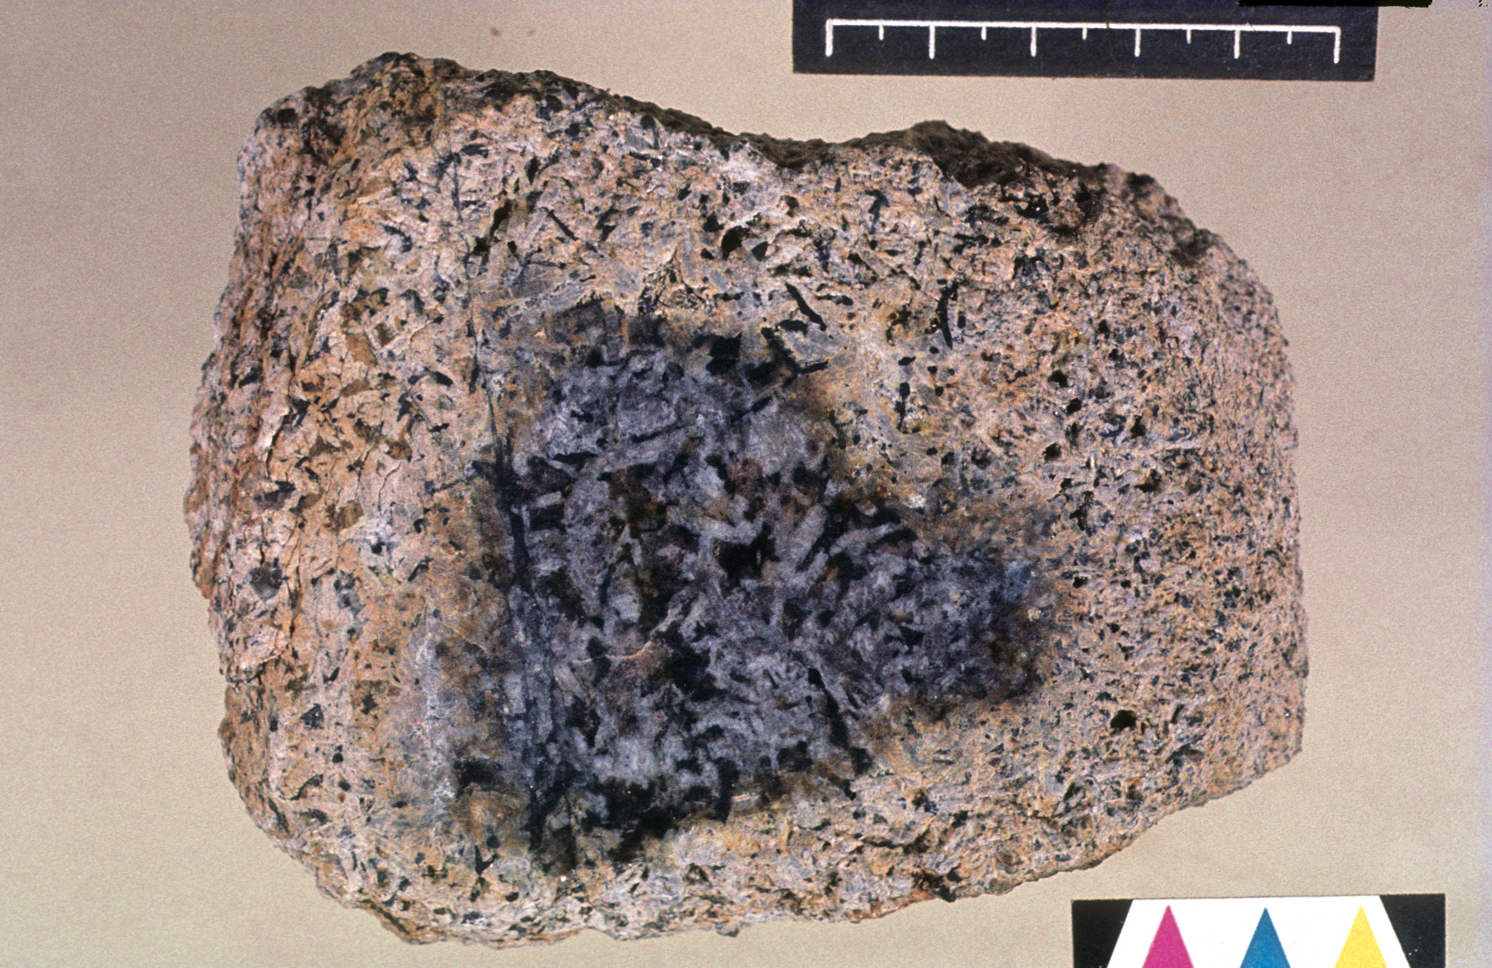
\includegraphics[width=\linewidth,height=4.6cm,keepaspectratio]{images/book1/bauxite.jpg}

{\small Bauxite, the \omterm{def:g5:raw-materials-and-recycling:raw-material}{ore} of aluminium, around a core of unweathered
rock. Photo: Werner Schellmann, CC BY-SA 2.5.}
\end{minipage}\hfill
\begin{minipage}[b]{0.48\linewidth}\centering
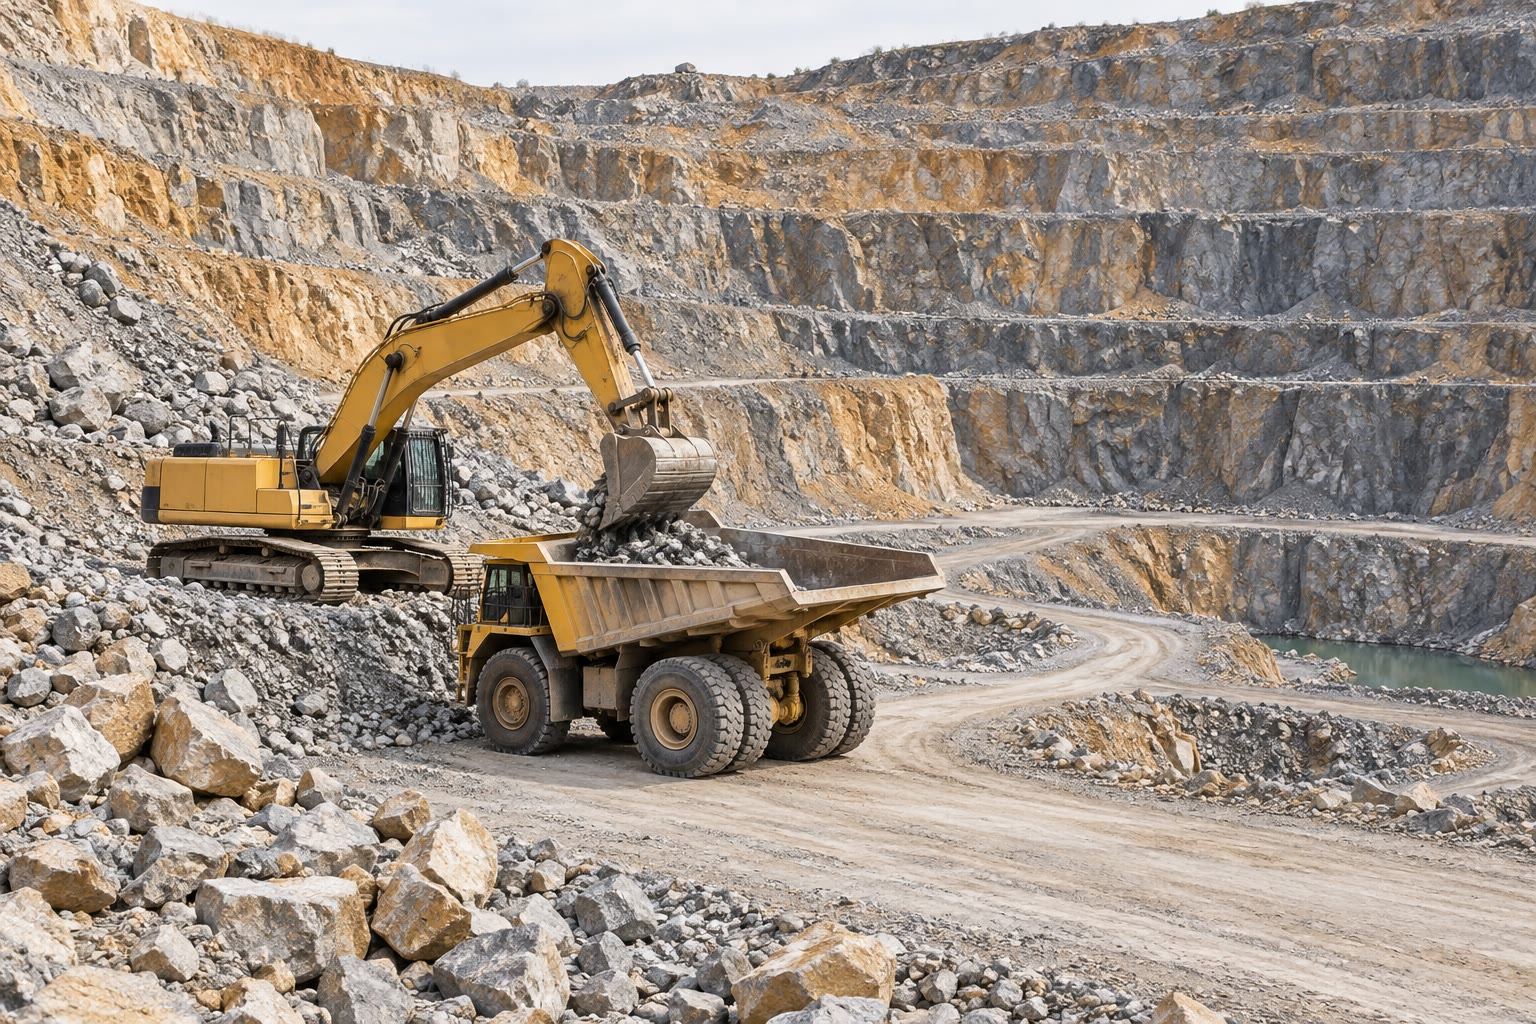
\includegraphics[width=\linewidth,height=4.6cm,keepaspectratio]{images/book1/ai/g5-quarry.jpg}

{\small A quarry: rock is dug out to be used as a \omterm{def:g5:raw-materials-and-recycling:raw-material}{raw material}.}
\end{minipage}
\end{omfigure}

\begin{omfigure}
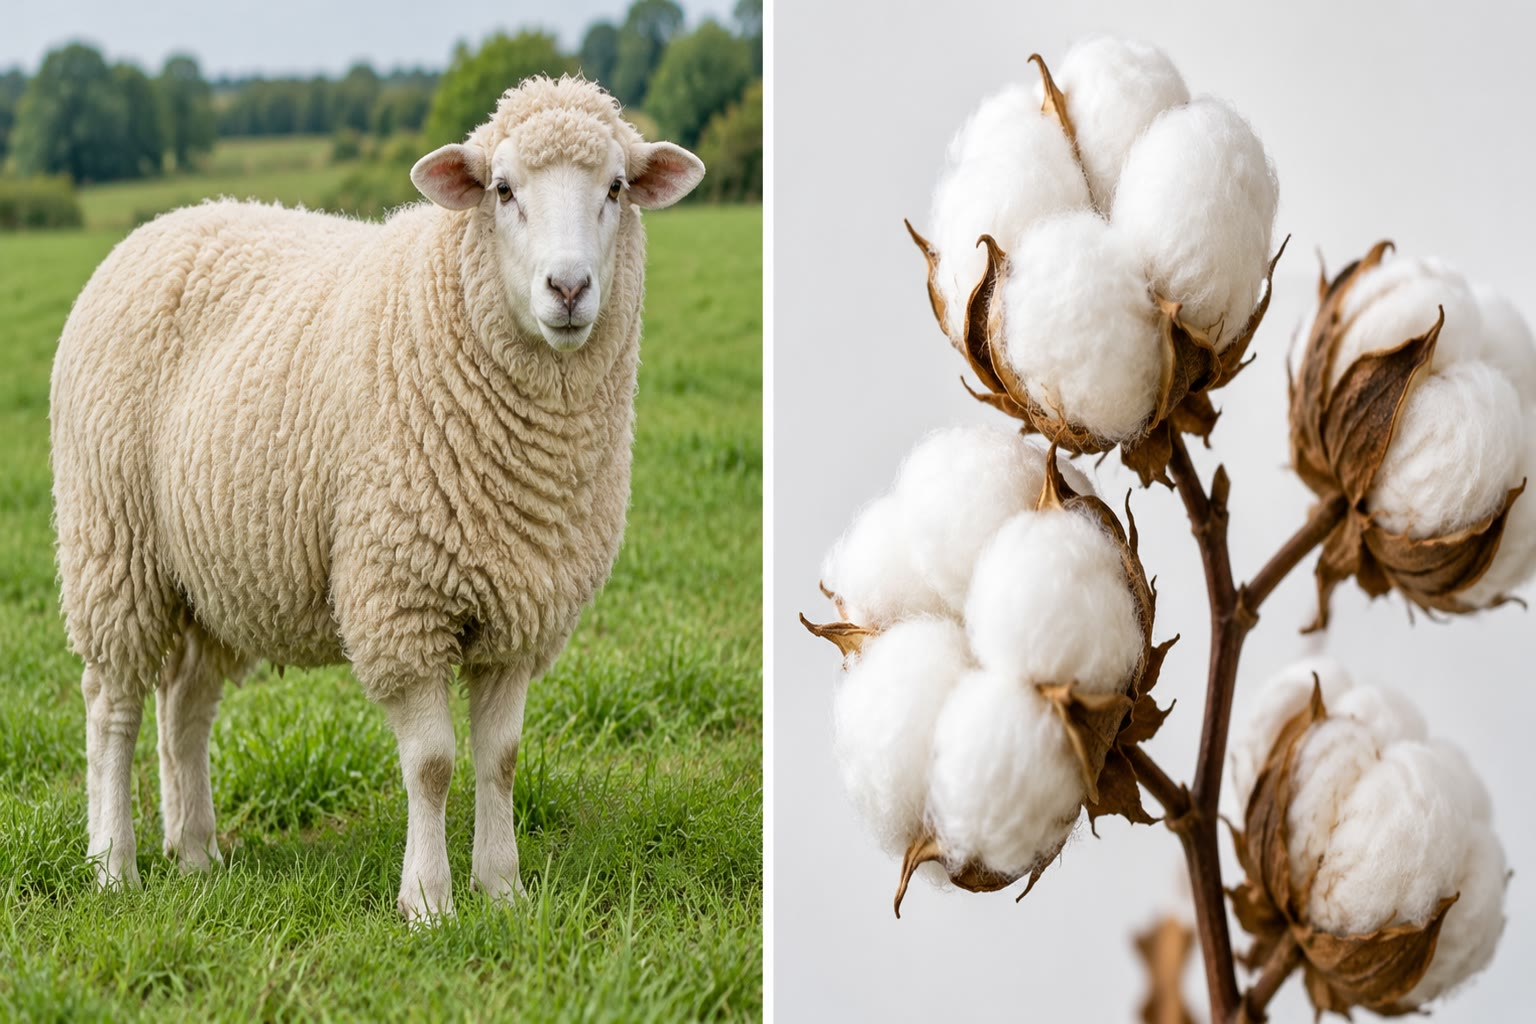
\includegraphics[width=0.6\linewidth]{images/book1/ai/g5-sheep-cotton.jpg}

{\small Natural \omterm{def:g5:raw-materials-and-recycling:raw-material}{raw materials} from living things: wool from sheep,
cotton from the cotton plant.}
\end{omfigure}

\section{From raw material to object}

\begin{proposition}[Making a material changes its raw material]\label{prop:g5:raw-materials-and-recycling:change}
Turning a \omterm{def:g5:raw-materials-and-recycling:raw-material}{raw material} into a \omterm{def:g5:raw-materials-and-recycling:natural-material}{manufactured material} takes energy ---
most often the heat of a furnace --- and usually \omterm{def:g5:irreversible-changes:chemical-change}{chemical changes}: sand
becomes glass, \omterm{def:g5:raw-materials-and-recycling:raw-material}{ore} becomes metal, oil becomes plastic. These changes
cannot simply be undone: glass does not turn back into sand.
\end{proposition}

\begin{example}[The life of a glass bottle]\label{ex:g5:raw-materials-and-recycling:bottle}
Sand, soda and crushed limestone are heated together in a furnace until
they melt into glass. The hot glass is blown into the shape of a bottle.
The bottle is filled, sold and emptied. Put in a bottle bank, it is
crushed into small pieces, melted again and blown into a new bottle:
the glass is used again and again.
\end{example}

\begin{omfigure}
\begin{tikzpicture}[font=\small,
    box/.style={draw=omDef, fill=omDef!6, rounded corners=2pt, align=center,
      minimum height=0.95cm, text width=2.4cm}]
  \node[box] (r) at (0,2.6) {raw material\\ (sand, ore, oil)};
  \node[box] (m) at (4.0,2.6) {making the\\ material};
  \node[box] (o) at (8.0,2.6) {object,\\ used};
  \node[box] (w) at (8.0,0) {waste};
  \node[box, draw=omProp, fill=omProp!8] (s) at (4.0,0) {sorting and\\ recycling};
  \draw[->, thick, omDef] (r) -- (m);
  \draw[->, thick, omDef] (m) -- (o);
  \draw[->, thick, omDef] (o) -- (w);
  \draw[->, thick, omProp] (w) -- (s);
  \draw[->, thick, omProp] (s) -- (m) node[midway, left, align=right, text=black]
    {used again\\ instead of new\\ raw material};
  \draw[->, thick, black!45, dashed] (w.east) -- ++(1.4,0) node[right, align=left,
    text=black] {thrown away:\\ landfill};
\end{tikzpicture}

{\small The life of a material. The orange loop is \omterm{def:g5:raw-materials-and-recycling:recycling}{recycling}: the
material of an old object replaces new \omterm{def:g5:raw-materials-and-recycling:raw-material}{raw material}.}
\end{omfigure}

\section{Sorting and recycling}

\begin{definition}[Recycling]\label{def:g5:raw-materials-and-recycling:recycling}
\emph{Recycling}\index{recycling} is collecting used objects and
treating their material so that it can be made into new objects,
instead of being thrown away.
\end{definition}

\begin{proposition}[Why recycle]\label{prop:g5:raw-materials-and-recycling:why}
% ledger: al:energy-primary, al:energy-recycled (8.3 / 186 = about 1/22)
\omterm{def:g5:raw-materials-and-recycling:recycling}{Recycling} saves \omterm{def:g5:raw-materials-and-recycling:raw-material}{raw materials}, which do not have to be dug out of the
ground, and it often saves energy. Making aluminium from old cans takes
only about one twentieth of the energy needed to make it from bauxite.
It also means less waste in landfills.
\end{proposition}

\begin{method}[Sorting waste for recycling]\label{met:g5:raw-materials-and-recycling:sort}
\omterm{def:g5:raw-materials-and-recycling:recycling}{Recycling} starts with sorting, wherever waste is thrown away:
\begin{enumerate}
  \item glass bottles and jars in one bin;
  \item metal cans, paper and card, and plastic bottles in the bins the
        town provides for them (the colours of the bins differ from
        place to place);
  \item what cannot be recycled with the rest of the waste.
\end{enumerate}
Each material is recycled in its own way, so a bin must hold only the
materials it is meant for.
\end{method}

\begin{omfigure}
\begin{tikzpicture}[font=\small]
  \foreach \k/\t/\bc in {0/glass/green!50!black, 1/{metal cans}/gray,
                        2/{paper and card}/omDef, 3/{plastic bottles}/orange!80!black} {
    \begin{scope}[xshift=\k*3.4cm]
      \fill[\bc!18, draw=\bc, line width=0.8pt] (-1,0) -- (1,0) -- (1.15,2.0)
        -- (-1.15,2.0) -- cycle;
      \fill[\bc!45, draw=\bc] (-1.25,2.0) rectangle (1.25,2.3);
      \node[anchor=north, align=center] at (0,-0.15) {\t};
    \end{scope}
  }
  % glass: a bottle
  \fill[green!40!black!60] (-0.2,0.3) rectangle (0.2,1.2);
  \fill[green!40!black!60] (-0.07,1.2) rectangle (0.07,1.6);
  % metal: a can
  \begin{scope}[xshift=3.4cm]
    \fill[black!25, draw=black!55] (-0.3,0.3) rectangle (0.3,1.3);
  \end{scope}
  % paper: a box and a sheet
  \begin{scope}[xshift=6.8cm]
    \fill[brown!25, draw=brown!60] (-0.6,0.3) rectangle (0.1,1.0);
    \fill[white, draw=black!40] (0.2,0.3) rectangle (0.65,1.3);
  \end{scope}
  % plastic: a bottle
  \begin{scope}[xshift=10.2cm]
    \fill[cyan!20, draw=cyan!50!black] (-0.25,0.3) rectangle (0.25,1.3);
    \fill[cyan!20, draw=cyan!50!black] (-0.1,1.3) rectangle (0.1,1.6);
  \end{scope}
\end{tikzpicture}

{\small Four sorting bins, one per material. (The colours of real bins
differ from town to town.)}
\end{omfigure}

\begin{omfigure}
\begin{minipage}[t]{0.48\linewidth}\centering
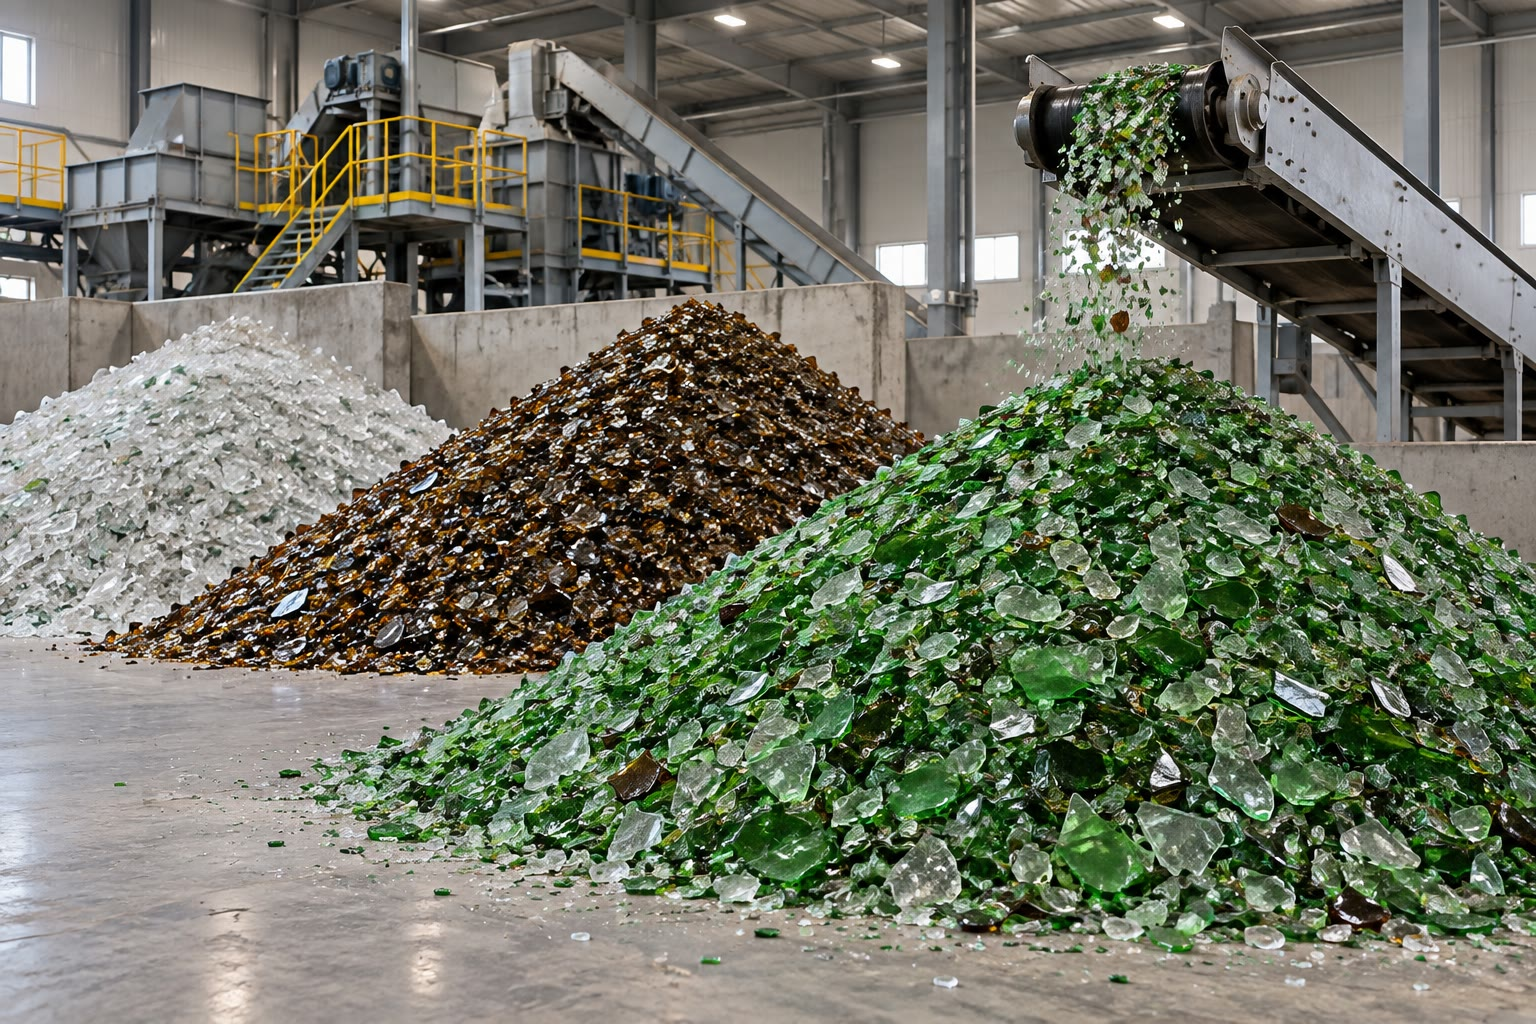
\includegraphics[width=\linewidth,height=4.6cm,keepaspectratio]{images/book1/ai/g5-glass-cullet.jpg}

{\small Crushed glass in a \omterm{def:g5:raw-materials-and-recycling:recycling}{recycling} plant, ready to be melted.}
\end{minipage}\hfill
\begin{minipage}[t]{0.48\linewidth}\centering
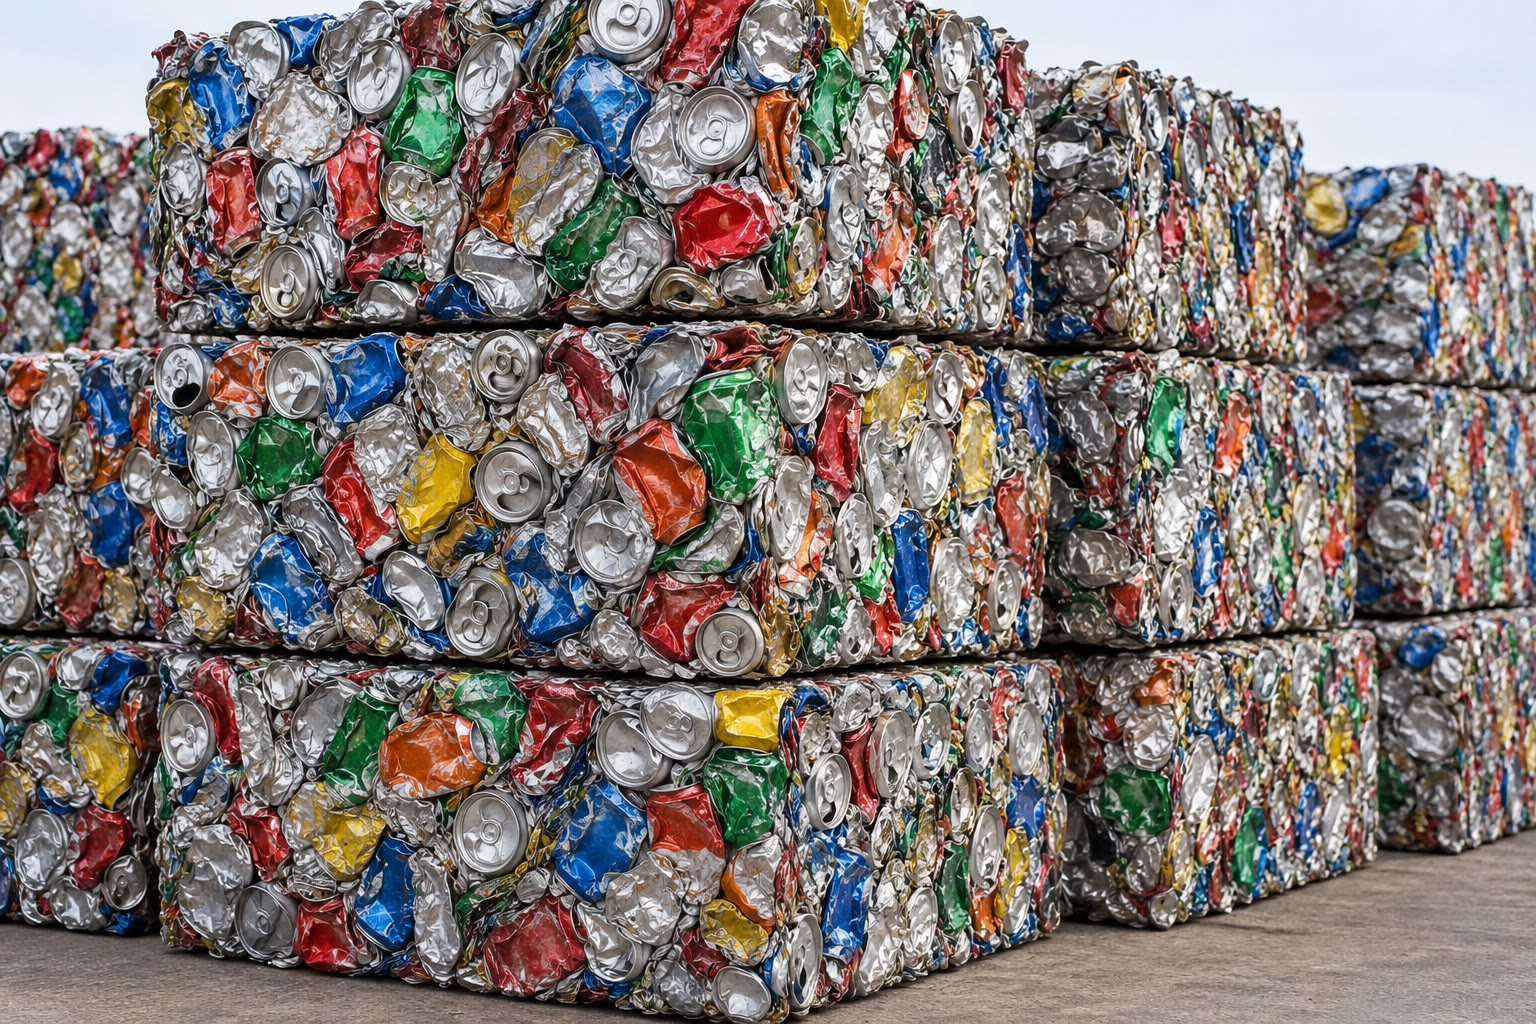
\includegraphics[width=\linewidth,height=4.6cm,keepaspectratio]{images/book1/ai/g5-can-bales.jpg}

{\small Bales of crushed aluminium cans.}
\end{minipage}
\end{omfigure}

\section{Waste and resources}

\begin{definition}[Resource]\label{def:g5:raw-materials-and-recycling:resource}
A \emph{resource}\index{resource} is anything taken from nature that
people use: water, wood, \omterm{def:g5:raw-materials-and-recycling:raw-material}{ores}, oil, sand. A \emph{renewable
resource}\index{renewable resource} grows back or comes back by itself
in a human lifetime, like wood from a forest that is replanted or wool
from sheep. \omterm{def:g5:raw-materials-and-recycling:raw-material}{Ores} and crude oil are not renewable: once they are dug out
and used, they are gone.
\end{definition}

\begin{proposition}[Reduce, reuse, recycle]\label{prop:g5:raw-materials-and-recycling:three}
To make \omterm{def:g5:raw-materials-and-recycling:resource}{resources} last, people can, in this order:
\begin{enumerate}
  \item \textbf{reduce}: use fewer objects, for instance fewer
        wrappings;
  \item \textbf{reuse}: use the same object again, like a glass jar
        refilled or a bag carried back to the shop;
  \item \textbf{recycle}: turn the material into a new object.
\end{enumerate}
\omterm{def:g5:raw-materials-and-recycling:recycling}{Recycling} comes last because it still needs energy and machines; the
best waste is the waste that is never made.
\end{proposition}

\section{Exercises}

\begin{exercise}[$\star$]\label{exo:g5:raw-materials-and-recycling:1}
Natural or manufactured? Wood, glass, wool, steel, plastic, stone.
\end{exercise}

\begin{exercise}[$\star$]\label{exo:g5:raw-materials-and-recycling:2}
Give the \omterm{def:g5:raw-materials-and-recycling:raw-material}{raw material} of: a sheet of paper, a glass jar, a cotton
T-shirt, a plastic bottle.
\end{exercise}

\begin{exercise}[$\star$]\label{exo:g5:raw-materials-and-recycling:3}
What is an \omterm{def:g5:raw-materials-and-recycling:raw-material}{ore}? Name the \omterm{def:g5:raw-materials-and-recycling:raw-material}{ore} of aluminium.
\end{exercise}

\begin{exercise}[$\star$]\label{exo:g5:raw-materials-and-recycling:4}
In which bin do you put: an empty jam jar, a newspaper, a drink can, a
plastic water bottle?
\end{exercise}

\begin{exercise}[$\star$]\label{exo:g5:raw-materials-and-recycling:5}
Look at the figure of the life of a material. What does the orange loop
replace?
\end{exercise}

\begin{exercise}[$\star$]\label{exo:g5:raw-materials-and-recycling:6}
Renewable or not: wood, crude oil, wool, iron \omterm{def:g5:raw-materials-and-recycling:raw-material}{ore}, cotton?
\end{exercise}

\begin{exercise}[$\star$]\label{exo:g5:raw-materials-and-recycling:7}
Why can glass not be turned back into sand by cooling it?
\end{exercise}

\begin{exercise}[$\star$]\label{exo:g5:raw-materials-and-recycling:8}
Give one way to reduce, one way to reuse and one way to recycle.
\end{exercise}

\begin{exercise}[$\star$]\label{exo:g5:raw-materials-and-recycling:9}
Why must a glass bin hold only glass?
\end{exercise}

\begin{exercise}[$\star\star$]\label{exo:g5:raw-materials-and-recycling:10}
Making aluminium from old cans needs about one twentieth of the energy
needed to make it from bauxite. A factory uses 20 units of energy to make
a batch of aluminium from bauxite. About how many units would it use to
make the same batch from old cans?
\end{exercise}

\begin{exercise}[$\star\star$]\label{exo:g5:raw-materials-and-recycling:11}
Why is ``reduce'' put before ``recycle''?
\end{exercise}
